%%%%%%%%%%%%%%%%%%%%%%%%%%%%%%%%%%%%%%%%%%%%%%%%%%%%%%%%%%%%%%%%%%%%%%%%
%% Draft as of July 9, 2002
%%%%%%%%%%%%%%%%%%%%%%%%%%%%%%%%%%%%%%%%%%%%%%%%%%%%%%%%%%%%%%%%%%%%%%%%

% For Phys. Rev. appearance, change preprint to twocolumn.
% Choose pra, prb, prc, prd, pre, prl, prstab, or rmp for journal
% Add 'draft' option to mark overfull boxes with black boxes
% Add 'showpacs' option to make PACS codes appear
% Add 'showkeys' option to make keywords appear

%\documentclass[aps,prl,preprint,groupedaddress]{revtex4}
\documentclass[aps,prl,twocolumn,groupedaddress]{revtex4}
%\documentclass[aps,prl,          groupedaddress]{revtex4}
%\documentclass[aps,prl,preprint,superscriptaddress]{revtex4}

\usepackage{graphicx}

\begin{document}

%%%%%%%%%%%%%% Begin Commands %%%%%%%%%%%%%%%%%%%%%%%%%%%%%%%%%%%%%%%%%%
\def\eps{\varepsilon}
\def\ms{\overline{\rm MS}}
\def\lms{\Lambda_{\ms}}
\def\disg{{\rm DIS}_\gamma}

\def\f2y{F_2^\gamma}
\def\fqy{f_{q/\gamma}}
\def\fby{f_{\bar{q}/\gamma}}
\def\fgy{f_{g/\gamma}}
\def\d  {{\rm d}}
\def\O  {{\cal O}}

\def\lp{\left. }
\def\rp{\right. }
\def\lr{\left( }
\def\rr{\right) }
\def\le{\left[ }
\def\re{\right] }
\def\lg{\left\{ }
\def\rg{\right\} }
\def\lb{\left| }
\def\rb{\right| }

\def\beq{\begin{equation}}
\def\eeq{\end{equation}}
\def\bea{\begin{eqnarray}}
\def\eea{\end{eqnarray}}
%%%%%%%%%%%%%% End of Commands %%%%%%%%%%%%%%%%%%%%%%%%%%%%%%%%%%%%%%%%%

%%%%%%%%%%%% Begin Cover Page %%%%%%%%%%%%%%%%%%%%%%%%%%%%%%%%%%%%%%%%%%
\preprint{DESY 02-052}
\preprint{FERMILAB-Pub-02/071-E}
\title{Strong Coupling Constant from the Photon Structure Function}
\author{Simon Albino}
\affiliation{{II.} Institut f\"ur Theoretische Physik, Universit\"at Hamburg,
             Luruper Chaussee 149, D-22761 Hamburg, Germany}
\author{Michael Klasen}
\email[]{michael.klasen@desy.de}
\affiliation{{II.} Institut f\"ur Theoretische Physik, Universit\"at Hamburg,
             Luruper Chaussee 149, D-22761 Hamburg, Germany}
\author{Stefan S\"oldner-Rembold}
\thanks{Heisenberg Fellow}
\affiliation{FNAL, P.O.\ Box 500, MS 357, Batavia, IL 60510, USA}
\date{\today}
\begin{abstract}
Abstract
\end{abstract}
\pacs{12.38.Bx,12.38.Qk,13.65.+i}
%     pQCD    ,exp.test,e+e-->HA
\maketitle
%%%%%%%%%%%% End of Cover Page %%%%%%%%%%%%%%%%%%%%%%%%%%%%%%%%%%%%%%%%%

%%%%%%%%%%%%%% Begin Main Body %%%%%%%%%%%%%%%%%%%%%%%%%%%%%%%%%%%%%%%%%



%%%%%%%%%%%%%% Begin Table I %%%%%%%%%%%%%%%%%%%%%%%%%%%%%%%%%%%%%%%%%%%
\begin{table}
\caption{\label{tab:1}$\chi^2$/DF and $\alpha_s(m_Z)$ values obtained in LO and
         NLO in the $\ms$ and $\disg$ factorization schemes with a
         single-parameter fit of
         the pointlike photon structure function $\f2y$. Also shown are the 
         results obtained without LEP data and with very high $Q^2$ data.}
\begin{ruledtabular}
\begin{tabular}{llc}
       Scheme & ~~~$\chi^2/$DF& $\alpha_s(m_Z)$ \\
\hline
       LO     & ~~7.9/~19& $0.1260\pm0.0055$(ex)$^{+0.0061}_{-0.0055}$(th) \\
       $\ms$  & ~~9.1/~19& $0.1183\pm0.0050$(ex)$^{+0.0029}_{-0.0028}$(th) \\
       $\disg$& ~~8.1/~19& $0.1195\pm0.0051$(ex)$^{+0.0031}_{-0.0028}$(th) \\
\hline
        w/o LEP &~~3.2/~~7& $0.1244\pm0.0126$(ex)$^{+0.0033}_{-0.0032}$(th) \\
        high $Q^2$ &~11.9/~~8& $0.1159\pm0.0125$(ex)$^{+0.0018}_{-0.0018}$(th) \\
\end{tabular}
\end{ruledtabular}
\end{table}
%%%%%%%%%%%%%% End of Table I %%%%%%%%%%%%%%%%%%%%%%%%%%%%%%%%%%%%%%%%%%
%


%
%%%%%%%%%%%%%% Begin Figure I %%%%%%%%%%%%%%%%%%%%%%%%%%%%%%%%%%%%%%%%%%
\begin{figure}
 \centering
 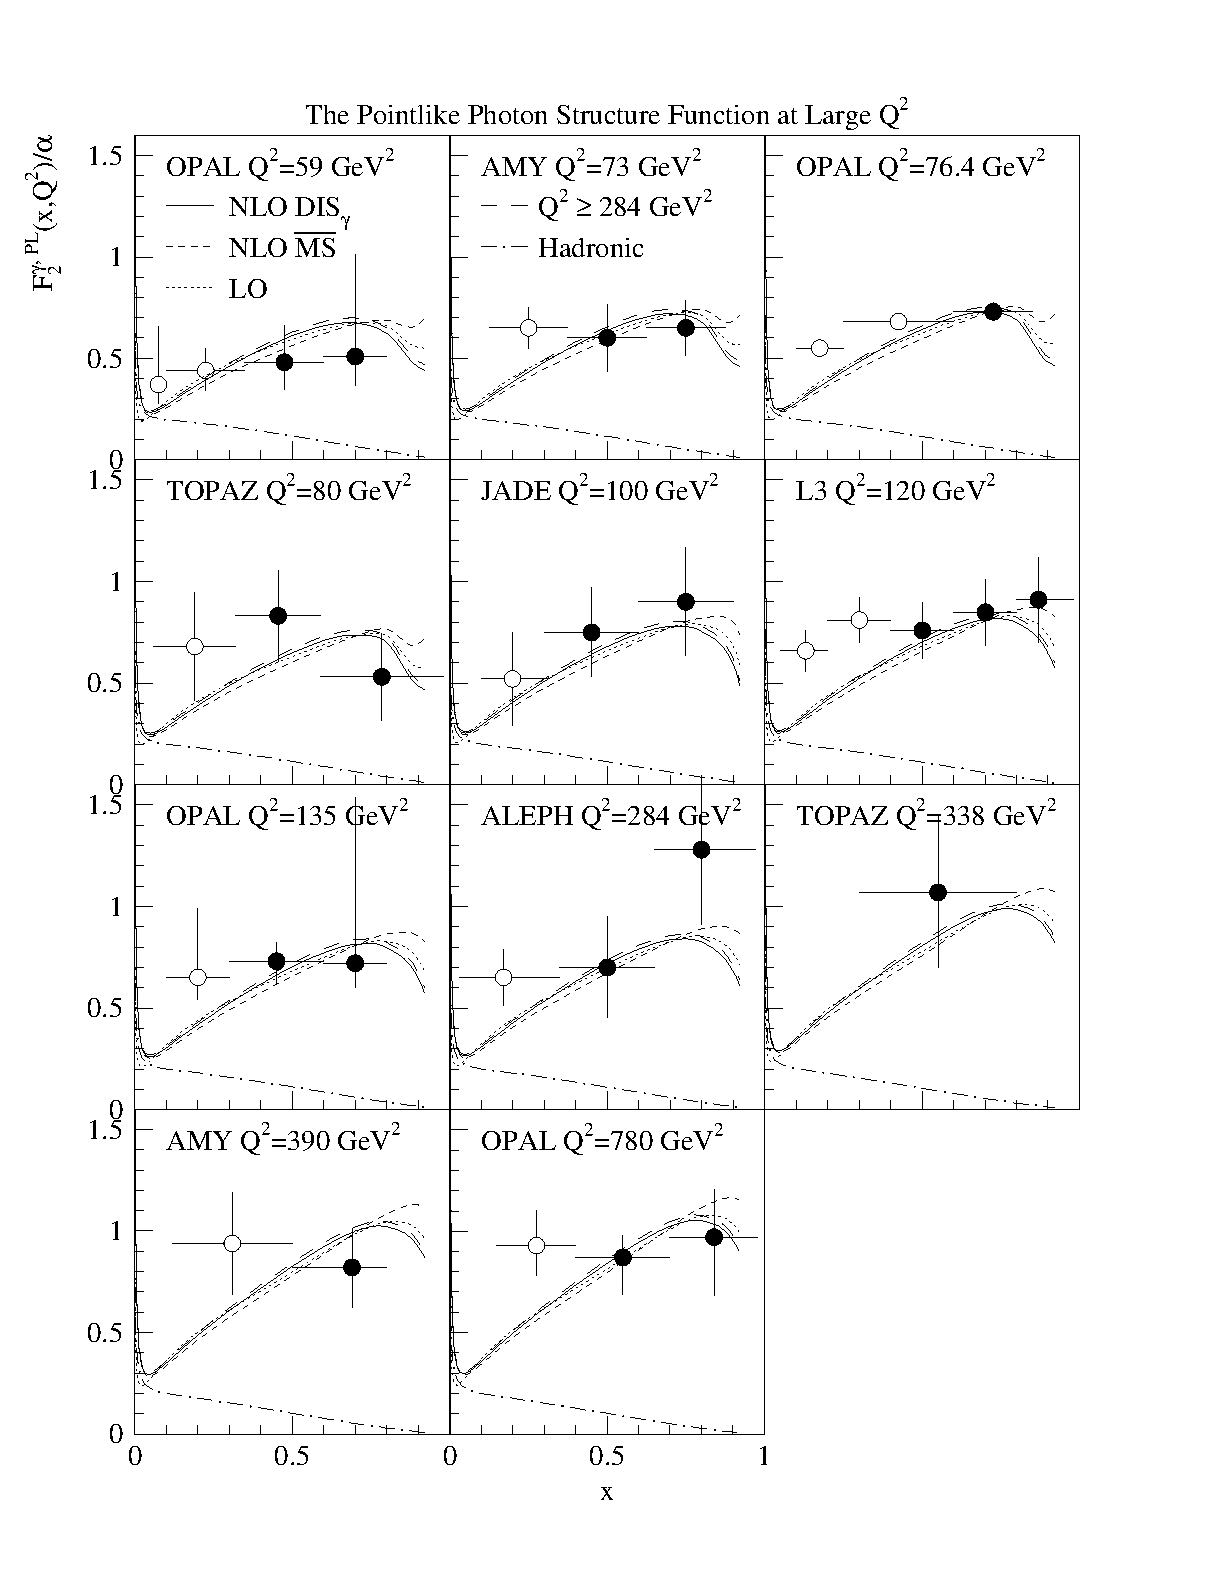
\includegraphics[width=0.9\columnwidth]{fig1}
 \caption{\label{fig:1}Single-parameter fits of the pointlike photon structure
 function, compared to PETRA \cite{Bartel:1984cg}, TRISTAN \cite{Sahu:1995gj,
 Muramatsu:1994rq}, and LEP \cite{Barate:1999qy,Acciarri:1998ig,
 Ackerstaff:1997ni,Ackerstaff:1997se,Abbiendi:2002te} data at large
 $Q^2$. The data points marked by open circles have not been used in
 the fits. Also shown is the hadronic contribution from a five-parameter NLO
 fit of the full photon structure function in the $\disg$ scheme.}
\end{figure}
%%%%%%%%%%%%%% End of Figure I %%%%%%%%%%%%%%%%%%%%%%%%%%%%%%%%%%%%%%%%%
%
.


%
%%%%%%%%%%%%%% Begin Table II %%%%%%%%%%%%%%%%%%%%%%%%%%%%%%%%%%%%%%%%%%
\begin{table}
\caption{\label{tab:2}$Q_0$, $\chi^2$/DF,
         and $\alpha_s(m_Z)$ values obtained in LO and
         NLO in the $\ms$ and $\disg$ factorization schemes with a
         five-parameter fit of
         the hadronic  photon structure function $\f2y$. Also shown are the 
         results obtained without LEP data.}
\begin{ruledtabular}
\begin{tabular}{lllc}
       Scheme & $Q_0$/GeV &~$\chi^2/$DF& $\alpha_s(m_Z)$ \\
\hline
       LO     & $0.79\pm0.18$&121/129& $0.1475\pm0.0074$(ex)$^{+0.0141}_{-0.0072}$(th)\\
       $\ms$  & $0.83\pm0.09$&118/129& $0.1198\pm0.0028$(ex)$^{+0.0034}_{-0.0046}$(th)\\
       $\disg$& $0.85\pm0.09$&115/129& $0.1216\pm0.0028$(ex)$^{+0.0033}_{-0.0050}$(th)\\
\hline
       w/o LEP& $0.46\pm0.10$&~37/~38& $0.1147\pm0.0047$(ex)$^{+0.0282}_{-0.0033}$(th)\\
\end{tabular}
\end{ruledtabular}
\end{table}
%%%%%%%%%%%%%% End of Table II %%%%%%%%%%%%%%%%%%%%%%%%%%%%%%%%%%%%%%%%%

%%%%%%%%%%%%%% Begin Figure II %%%%%%%%%%%%%%%%%%%%%%%%%%%%%%%%%%%%%%%%%
\begin{figure}
 \centering
 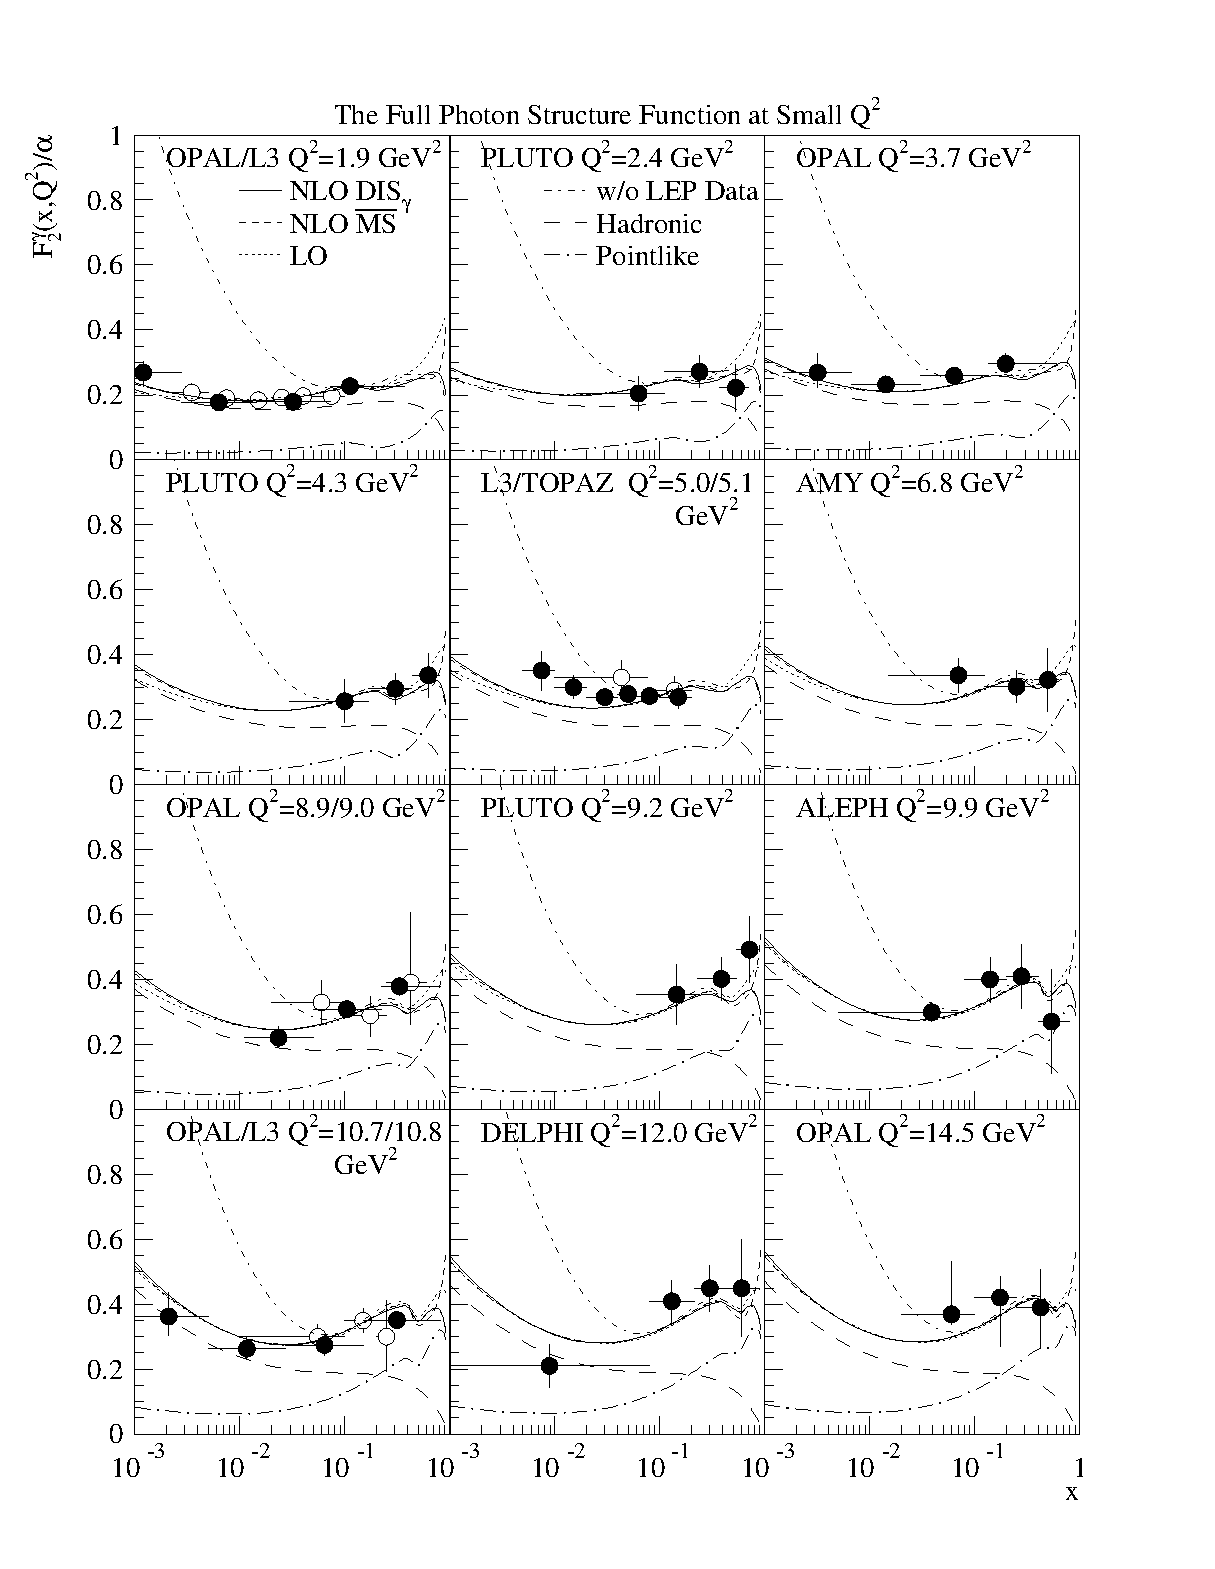
\includegraphics[width=0.9\columnwidth]{fig2}
 \caption{\label{fig:2}Five-parameter fits of the full photon structure
 function, compared to data from PETRA \cite{Berger:1984xt}, TRISTAN
 \cite{Kojima:1997wg,Muramatsu:1994rq}, and LEP \cite{Barate:1999qy,
 Abreu:1996xt,Acciarri:1998ig,%Acciarri:1999bh,
 Ackerstaff:1997ni,
 Abbiendi:2000cw} at small $Q^2$. The data points marked by open
 circles refer to the second experiment and/or $Q^2$ value. Also shown are the
 hadronic and pointlike contributions to the NLO fit in the $\disg$ scheme.}
\end{figure}
%%%%%%%%%%%%%% End of Figure II %%%%%%%%%%%%%%%%%%%%%%%%%%%%%%%%%%%%%%%%
%
we compare our results to the fitted $\f2y$ data in the region of low $x$
and $Q^2$. This region is clearly dominated by the hadronic contribution
and by the impact of the LEP data. A fit without the LEP data results in a rise
of $\f2y$ at low $x$, which is much too steep. The fits are perturbatively
stable and the data are described almost equally well in the $\ms$ and $\disg$
scheme.

Since the total error on $\alpha_s(m_Z)$ is smaller in the full fit than in
the pointlike fit due to the larger number of data points, we adopt as our
final result
\pagebreak
\beq
 \alpha_s(m_Z)=0.1198\pm0.0054
\eeq
in NLO and the $\ms$ scheme, where the larger theoretical error has been added
to the experimental error in quadrature. While our total error is
slightly larger than those obtained in $Z$-boson- and
$\tau$-decays at LEP, it is comparable to the errors obtained in deep-inelastic
scattering at HERA and heavy quarkonium decays. This encourages us to
combine our result with the current world average of $0.1172\pm0.0014$
\cite{Groom:2000in} to a new world average
\beq
 \alpha_s(m_Z)=0.1175\pm0.0014,
\eeq
where the errors are assumed to be uncorrelated.

In conclusion, we have for the first time fitted the now final PETRA,
TRISTAN, and LEP data on the photon structure function $\f2y$ in NLO of
perturbative QCD. We have extracted the value of the strong coupling constant
$\alpha_s(m_Z)$ with competitive experimental and theoretical errors from a
single-parameter pointlike fit to data at large $x$ and $Q^2$ and from a
five-parameter full (pointlike and hadronic) fit at all $x$ and $Q^2$.
Our analysis proves that the available $\f2y$ data contribute significantly
to a precise determination of $\alpha_s$ and that future measurements of
$\f2y$ at linear colliders will have a large impact.

%%%%%%%%%%%%%% End of Main Body %%%%%%%%%%%%%%%%%%%%%%%%%%%%%%%%%%%%%%%%

%%%%%%%%%%%%%% Begin Acknowledgment %%%%%%%%%%%%%%%%%%%%%%%%%%%%%%%%%%%%
\begin{acknowledgments}

We thank G.\ Kramer for many valuable discussions and a careful reading of the
manuscript. S.\ A.\ and M.\ K.\ are supported by the Deutsche
Forschungsgemeinschaft through Grant No.\ KL~1266/1-2. % and by the European
%Commission through Grant No.\ ERBFMRX-CT98-0194.

\end{acknowledgments}
%%%%%%%%%%%%%% End of Acknowledgment %%%%%%%%%%%%%%%%%%%%%%%%%%%%%%%%%%%

%%%%%%%%%%%%%% Begin References %%%%%%%%%%%%%%%%%%%%%%%%%%%%%%%%%%%%%%%%
\begin{thebibliography}{1}

%%% PDG REVIEW %%%

%\cite{Groom:2000in}
\bibitem{Groom:2000in}
%D.~Groom {\it et al.}, %  [Particle Data Group Collaboration],
K.~Hagiwara {\it et al.},
%``Review of particle physics,''
%Eur.\ Phys.\ J.\ C {\bf 15} (2000) 1.
Phys.\ Rev.\ D {\bf 66} (2002) 010001.
%and 2001 off-year partial update for the 2002 edition available on the PDG WWW
%pages (URL: http://pdg.lbl.gov/).
%%CITATION = EPHJA,C15,1;%%

%%% POINTLIKE PHOTON %%%

%\cite{Witten:1977ju}
\bibitem{Witten:1977ju}
E.~Witten,
%``Anomalous Cross-Section For Photon - Photon Scattering In Gauge Theories,''
Nucl.\ Phys.\ B {\bf 120} (1977) 189.
%%CITATION = NUPHA,B120,189;%%

%\cite{Bardeen:1979hg}
\bibitem{Bardeen:1979hg}
W.~Bardeen and A.~Buras,
%``Higher Order Asymptotic Freedom Corrections To Photon - Photon Scattering,''
Phys.\ Rev.\ D {\bf 20} (1979) 166; {\bf 21} (1979) 2041(E).
%%CITATION = PHRVA,D20,166;%%

%\cite{Duke:1980ij}
\bibitem{Duke:1980ij}
D.~Duke and J.~Owens,
%``The Photon Structure Function As Calculated Using Perturbative Quantum Chromodynamics,''
Phys.\ Rev.\ D {\bf 22} (1980) 2280.
%%CITATION = PHRVA,D22,2280;%%

%\cite{Rossi:1983bp}
\bibitem{Rossi:1983bp}
G.~Rossi,
%``Singularities In The Perturbative QCD Treatment Of The Photon Structure Functions,''
Phys.\ Lett.\ B {\bf 130} (1983) 105.
%%CITATION = PHLTA,B130,105;%%

%\cite{Antoniadis:1983fv}
\bibitem{Antoniadis:1983fv}
I.Antoniadis, G.Grunberg,
%``Second Order QCD Analysis Of The Photon Structure Function,''
Nucl.\ Phys.\ B {\bf 213} (1983) 445.
%%CITATION = NUPHA,B213,445;%%

%\cite{Field:1986gf}
\bibitem{Field:1986gf}
J.Field,F.Kapusta,L.Poggioli,
%``On The Sensitivity Of The F(2) Photon Structure Function To The QCD Scale Parameter Lambda,''
Phys.Lett.B{\bf 181}(1986)362.
%%CITATION = PHLTA,B181,362;%%

%\cite{Frazer:1987sb}
\bibitem{Frazer:1987sb}
W.~Frazer,
%``Sensitivity Of The Photon Structure Function F2 To The QCD Scale Parameter Lambda,''
Phys.\ Lett.\ B {\bf 194} (1987) 287.
%%CITATION = PHLTA,B194,287;%%

%\cite{Gluck:1983mm}
\bibitem{Gluck:1983mm}
M.~Gl\"uck and E.~Reya,
%``Boundary Conditions For The Photon Structure Function In The Leading And Subleading Order,''
Phys.\ Rev.\ D {\bf 28} (1983) 2749;
%%CITATION = PHRVA,D28,2749;%%
%\cite{Rossi:1984xz}
%\bibitem{Rossi:1984xz}
G.~Rossi,
%``X Space Analysis For The Photon Structure Functions In QCD,''
{\it ibid.}
%Phys.\ Rev.\ D
{\bf 29} (1984) 852.
%%CITATION = PHRVA,D29,852;%%

%\cite{DeWitt:1979wn}
\bibitem{DeWitt:1979wn}
R.~DeWitt, L.~Jones, J.~Sullivan, D.~Willen and H.~Wyld,
%``Anomalous Components Of The Photon Structure Functions,''
Phys.\ Rev.\ D {\bf 19} (1979) 2046; {\bf 20} (1979) 1751(E).
%%CITATION = PHRVA,D19,2046;%%

%\cite{Wagner:1986dj}
\bibitem{Wagner:1986dj}
W.~Wagner,
%``Experimental Review Of The Photon Structure Function,''
UCD-86-29,
%{\it Talk given at 23rd Int. Conf. on High Energy Physics, Berkeley, CA, July 16-23, 1986}.
XXIII ICHEP, Berkeley (1986).

%%% OLD RPP ISSUES %%%

%\cite{Yost:1988ke}
\bibitem{Yost:1988ke}
G.~Yost {\it et al.},
%``Review Of Particle Properties: Particle Data Group,''
Phys.\ Lett.\ B {\bf 204} (1988) 1.
%%CITATION = PHLTA,B204,1;%%

%\cite{Hernandez:1990yc}
\bibitem{Hernandez:1990yc}
J.~Hernandez {\it et al.},
%``Review Of Particle Properties. Particle Data Group,''
Phys.\ Lett.\ B {\bf 239} (1990) 1; {\bf 253} (1990) 524(E).
%%CITATION = PHLTA,B239,1;%%

%\cite{Hikasa:1992je}
\bibitem{Hikasa:1992je}
K.~Hikasa {\it et al.}, %  [Particle Data Group Collaboration],
%``Review of particle properties. Particle Data Group,''
Phys.\ Rev.\ D {\bf 45} (1992) S1; {\bf 46} (1992) 5210(E).
%%CITATION = PHRVA,D45,S1;%%

%\cite{Montanet:1994xu}
\bibitem{Montanet:1994xu}
L.~Montanet {\it et al.}, %  [Particle Data Group Collaboration],
%``Review of particle properties. Particle Data Group,''
Phys.\ Rev.\ D {\bf 50} (1994) 1173.
%%CITATION = PHRVA,D50,1173;%%

%%% OTHER PDFS %%%

%\cite{Gluck:1992jc}
\bibitem{Gluck:1992jc}
M.Gl\"uck, E.Reya, A.Vogt,
%``Photonic parton distributions,''
Phys.\ Rev.\ D {\bf 46} (1992) 1973.
%%CITATION = PHRVA,D46,1973;%%

%\cite{Aurenche:1994in}
\bibitem{Aurenche:1994in}
P.~Aurenche, M.~Fontannaz and J.~P.~Guillet,
%``Parton distributions in the photon,''
Z.\ Phys.\ C {\bf 64} (1994) 621.
%[arXiv:hep-ph/9406382].
%%CITATION = HEP-PH 9406382;%%

%\cite{Schuler:1995fk}
\bibitem{Schuler:1995fk}
G.~Schuler and T.~Sj\"ostrand,
%``Low and high mass components of the photon distribution functions,''
Z.\ Phys.\ C {\bf 68} (1995) 607.
%[arXiv:hep-ph/9503384].
%%CITATION = HEP-PH 9503384;%%

%\cite{Gordon:1997pm}
\bibitem{Gordon:1997pm}
L.~Gordon and J.~Storrow,
%``New parton distribution functions for the photon,''
Nucl.\ Phys.\ B {\bf 489} (1997) 405.
%[arXiv:hep-ph/9607370].
%%CITATION = HEP-PH 9607370;%%

%\cite{Gluck:1999ub}
\bibitem{Gluck:1999ub}
M.~Gl\"uck, E.~Reya and I.~Schienbein,
%``Radiatively generated parton distributions of real and virtual photons,''
Phys.\ Rev.\ D {\bf 60} (1999) 054019; {\bf 62} (1999) 019902(E).
%[arXiv:hep-ph/9903337].
%%CITATION = HEP-PH 9903337;%%

%%% FFNS %%%

%\cite{Gluck:1992ee}
\bibitem{Gluck:1992ee}
M.Gl\"uck, E.Reya, A.Vogt,
%``Parton structure of the photon beyond the leading order,''
Phys.\ Rev.\ D {\bf 45} (1992) 3986.
%%CITATION = PHRVA,D45,3986;%%

%%% LO BETHE-HEITLER CROSS SECTION %%%

%\cite{Budnev:1974de}
\bibitem{Budnev:1974de}
V.~Budnev, I.~Ginzburg, G.~Meledin and V.~Serbo,
%``The Two Photon Particle Production Mechanism. Physical Problems. Applications. Equivalent Photon Approximation,''
Phys.\ Rept.\  {\bf 15} (1974) 181.
%%CITATION = PRPLC,15,181;%%

%%% NLO BETHE-HEITLER CROSS SECTION %%%

%\cite{Laenen:1994ce}
\bibitem{Laenen:1994ce}
E.~Laenen, S.~Riemersma, J.~Smith and W.~van Neerven,
%``Complete next-to-leading order QCD corrections to the photon structure functions F2 (gamma) (x, Q**2) and F-L (gamma) (x, Q**2),''
Phys.\ Rev.\ D {\bf 49} (1994) 5753.
%[arXiv:hep-ph/9308295].
%%CITATION = HEP-PH 9308295;%%

%%% CHARM QUARK MASS %%%

%\cite{Kuhn:2001dm}
\bibitem{Kuhn:2001dm}
J.K\"uhn, M.Steinhauser,
%``Determination of alpha(s) and heavy quark masses from recent  measurements of R(s),''
Nucl.\ Phys.\ B {\bf 619} (2001) 588.
%[arXiv:hep-ph/0109084].
%%CITATION = HEP-PH 0109084;%%

%%% MINUIT %%%

%\cite{James:1975dr}
\bibitem{James:1975dr}
F.~James, M.~Roos,
%``'Minuit' A System For Function Minimization And Analysis Of The Parameter Errors And Correlations,''
Comp.\ Phys.\ Comm.\  {\bf 10} (1975) 343.
%%CITATION = CPHCB,10,343;%%

%%% PETRA F2GAMMA MEASUREMENTS %%%

%\cite{Bartel:1984cg}
\bibitem{Bartel:1984cg}
W.~Bartel {\it et al.}, % [JADE Collaboration],
%``Experimental Study Of The Photon Structure Function F(2) At Q**2 From 10-Gev**2 To 220-Gev**2,''
Z.\ Phys.\ C {\bf 24} (1984) 231.
%%CITATION = ZEPYA,C24,231;%%

%\cite{Berger:1984xt}
\bibitem{Berger:1984xt}
C.~Berger {\it et al.}, % [PLUTO Collaboration],
%``Measurement Of The Photon Structure Function F2 (X, Q**2),''
Phys.\ Lett.\ B {\bf 142} (1984) 111;
%%CITATION = PHLTA,B142,111;%%
%\cite{Berger:1987ke}
%\bibitem{Berger:1987ke}
%C.~Berger {\it et al.}, %  [PLUTO Collaboration],
%``Measurement And QCD Analysis Of The Photon Structure Function F2 (X, Q**2),''
Nucl.\ Phys.\ B {\bf 281} (1987) 365.
%%CITATION = NUPHA,B281,365;%%

%\cite{Althoff:1986fi}
\bibitem{Althoff:1986fi}
M.~Althoff {\it et al.}, %  [TASSO Collaboration],
%``Measurement Of The Photon Structure Function F2 (Gamma) At Q**2 From 7-Gev/C**2 To 70-Gev/C**2,''
Z.\ Phys.\ C {\bf 31} (1986) 527.
%%CITATION = ZEPYA,C31,527;%%

%%% TRISTAN F2GAMMA MEASUREMENTS %%%

%\cite{Sahu:1995gj}
\bibitem{Sahu:1995gj}
S.~Sahu {\it et al.}, %  [AMY Collaboration],
%``A High Q**2 measurement of the photon structure function F2(gamma),''
Phys.\ Lett.\ B {\bf 346} (1995) 208.
%%CITATION = PHLTA,B346,208;%%

%\cite{Kojima:1997wg}
\bibitem{Kojima:1997wg}
T.~Kojima {\it et al.}, %  [AMY Collaboration],
%``A measurement of the photon structure function F2(gamma) at  Q**2 = 6.8-GeV**2,''
Phys.\ Lett.\ B {\bf 400} (1997) 395.
%%CITATION = PHLTA,B400,395;%%

%\cite{Muramatsu:1994rq}
\bibitem{Muramatsu:1994rq}
K.~Muramatsu {\it et al.}, %  [TOPAZ Collaboration],
%``Measurement of the photon structure function F2(gamma) and jet production at TRISTAN,''
Phys.\ Lett.\ B {\bf 332} (1994) 477.
%%CITATION = PHLTA,B332,477;%%

%%% LEP F2GAMMA MEASUREMENTS %%%

%\cite{Barate:1999qy}
\bibitem{Barate:1999qy}
R.~Barate {\it et al.}, %  [ALEPH Collaboration],
%``Measurement of the hadronic photon structure function at LEP1 for   values between 9.9-GeV**2 and 284-GeV**2,''
Phys.\ Lett.\ B {\bf 458} (1999) 152.
%%CITATION = PHLTA,B458,152;%%

%\cite{Abreu:1996xt}
\bibitem{Abreu:1996xt}
P.~Abreu {\it et al.}, %  [DELPHI Collaboration],
%``A Measurement of the photon structure function F2(gamma) at an average Q**2 of 12-GeV**2/c**4,''
Z.\ Phys.\ C {\bf 69} (1996) 223.
%%CITATION = ZEPYA,C69,223;%%

%\cite{Acciarri:1998ig}
\bibitem{Acciarri:1998ig}
M.~Acciarri {\it et al.}, %  [L3 Collaboration],
%``Study of the hadronic photon structure function F2(gamma) at LEP,''
Phys.\ Lett.\ B {\bf 436} (1998) 403;
%%CITATION = PHLTA,B436,403;%%
%\cite{Acciarri:1999bh}
%\bibitem{Acciarri:1999bh}
%M.~Acciarri {\it et al.}, %  [L3 Collaboration],
%``The Q**2 evolution of the hadronic photon structure function F2(gamma)  at LEP,''
{\it ibid.},
%Phys.\ Lett.\ B
{\bf 447} (1999) 147;
%%CITATION = PHLTA,B447,147;%%
%\cite{Acciarri:2000rw}
%\bibitem{Acciarri:2000rw}
%M.~Acciarri {\it et al.}, %  [L3 Collaboration],
%``Measurement of the photon structure function at high Q**2 at LEP,''
{\it ibid.}, 
%Phys.\ Lett.\ B
{\bf 483} (2000) 373.
%[arXiv:hep-ex/0004005].
%%CITATION = HEP-EX 0004005;%%

%\cite{Ackerstaff:1997ni}
\bibitem{Ackerstaff:1997ni}
K.~Ackerstaff {\it et al.}, %  [OPAL Collaboration],
%``Measurement of the Q**2 evolution of the photon structure function  F2(gamma),''
Phys.\ Lett.\ B {\bf 411} (1997) 387.
%[arXiv:hep-ex/9708019].
%%CITATION = HEP-EX 9708019;%%

%\cite{Ackerstaff:1997se}
\bibitem{Ackerstaff:1997se}
K.~Ackerstaff {\it et al.}, %  [OPAL Collaboration],
%``Analysis of hadronic final states and the photon structure function  F2(gamma) in deep inelastic electron photon scattering at LEP,''
Z.\ Phys.\ C {\bf 74} (1997) 33.
%%CITATION = ZEPYA,C74,33;%%

%\cite{Abbiendi:2000cw}
\bibitem{Abbiendi:2000cw}
G.~Abbiendi {\it et al.}, %  [OPAL Collaboration],
%``Measurement of the low-x behavior of the photon structure function  F2(gamma),''
Eur.\ Phys.\ J.\ C {\bf 18} (2000) 15.
%[arXiv:hep-ex/0007018].
%%CITATION = HEP-EX 0007018;%%

%\cite{Abbiendi:2002te}
\bibitem{Abbiendi:2002te}
G.~Abbiendi {\it et al.}, %  [OPAL Collaboration],
%``Measurement of the hadronic photon structure function F2(gamma) at  LEP2,''
arXiv:hep-ex/0202035.
%%CITATION = HEP-EX 0202035;%%

%%% PEP F2GAMMA MEASUREMENTS %%%

%\cite{Aihara:1987xq}
\bibitem{Aihara:1987xq}
H.~Aihara {\it et al.}, %  [TPC/2$\gamma$ Collaboration],
%``Observation Of Scaling Of The Photon Structure Function F2 (Gamma) At Low Q**2,''
Phys.\ Rev.\ Lett.\  {\bf 58} (1987) 97.
%%CITATION = PRLTA,58,97;%%

%\cite{Aihara:1987xw}
\bibitem{Aihara:1987xw}
H.~Aihara {\it et al.}, %  [TPC/2$\gamma$ Collaboration],
%``Measurement Of The Photon Structure Function F2 (Gamma) (X, Q**2) In The Region 0.2-Gev**2 < 7-Gev**2,''
Z.\ Phys.\ C {\bf 34} (1987) 1.
%%CITATION = ZEPYA,C34,1;%%

%%% HIGH VALUE OF Q0 %%%

%\cite{Gordon:1994mu}
\bibitem{Gordon:1994mu}
L.Gordon,D.Holling,J.Storrow,
%``The Region of validity of perturbative QCD for the photon structure function F2 (gamma) (x, Q**2),''
J.\ Phys.\ G {\bf 20} (1994) 549.
%%CITATION = JPHGB,G20,549;%%

%%% GLUON FROM H1 DIJETS %%%

%\cite{Adloff:2000bs}
\bibitem{Adloff:2000bs}
C.~Adloff {\it et al.}, %  [H1 Collaboration],
%``Measurement of di-jet cross-sections in photoproduction and photon  structure,''
Phys.\ Lett.\ B {\bf 483} (2000) 36.
%[arXiv:hep-ex/0003011].
%%CITATION = HEP-EX 0003011;%%

\end{thebibliography}
%%%%%%%%%%%%%% End of References %%%%%%%%%%%%%%%%%%%%%%%%%%%%%%%%%%%%%%%

\end{document}
